\documentclass[lang=cn,newtx,10pt,scheme=chinese]{../../../elegantbook}

\title{基础提高练习题}
\subtitle{北街学长倾力之作}

\author{北街}
% \institute{Elegant\LaTeX{} Program}
\date{2022/12/31}
\version{1.0}
% \bioinfo{自定义}{信息}

% \extrainfo{注意:本模板自 2023 年 1 月 122222 日开始,不再更新和维护!}

\setcounter{tocdepth}{3}

\logo{../../figure/logo-blue.png}
\cover{../../figure/cover.jpg}

% 本文档命令
\usepackage{array}
\newcommand{\ccr}[1]{\makecell{{\color{#1}\rule{1cm}{1cm}}}}

% 修改标题页的橙色带
\definecolor{customcolor}{RGB}{32,178,170}
\colorlet{coverlinecolor}{customcolor}
\usepackage{cprotect}

\addbibresource[location=local]{reference.bib} % 参考文献,不要删除
\usepackage{listings}         % 导入listings宏包
\usepackage{xcolor}           % 支持颜色

% 配置C++代码样式
\lstset{
    language=C++,             % 语言设置为C++
    basicstyle=\ttfamily,      % 基本样式
    keywordstyle=\color{blue}, % 关键词颜色
    commentstyle=\color{green},% 注释颜色
    stringstyle=\color{red},   % 字符串颜色
    numbers=left,              % 显示行号
    numberstyle=\tiny,         % 行号样式
    stepnumber=1,              % 每行显示行号
    breaklines=true,           % 自动换行
    frame=lines                % 代码块边框样式
}
\begin{document}

\maketitle
\frontmatter

\tableofcontents

\mainmatter





\chapter{树与散列}


\begin{enumerate}
    \item 在任意一棵非空平衡二叉树(AVL 树)$T_1$ 中,删除某结点 $w$ 之后形成平衡二叉树 $T_2$,再将 $w$ 插入 $T_2$ 形成平衡二叉树 $T_3$。下列关于 $T_1$ 与 $T_3$ 的叙述中,正确的是( )。  
    【2019 年全国试题 4(2 分)】  

    A. 仅 I \\  
    B. 仅 II \\  
    C. 仅 I、II \\  
    D. 仅 II、III \\  

    答案:\textcolor{red}{C}

    解析:\\
    平衡二叉树(AVL 树)在插入或删除节点后可能需要通过旋转操作来保持平衡。分析三个选项:\\
    1. I. 若 $w$ 是 $T_1$ 的叶结点,则 $T_1$ 与 $T_3$ 可能不相同:\\
       删除叶结点后,可能引发树的重新平衡(旋转操作)。再插入时,树的结构可能发生变化。例如,删除叶结点后,树的高度可能减少,重新插入时,树的平衡因子可能发生变化,导致旋转操作。因此,$T_1$ 与 $T_3$ 可能不相同,该选项正确。\\
    2. II. 若 $w$ 不是 $T_1$ 的叶结点,则 $T_1$ 与 $T_3$ 一定不相同:\\
       删除非叶结点时,通常需要用其前驱或后继节点替代,这会改变树的结构。重新插入 $w$ 时,$w$ 的位置可能与原来不同,树的形态一定发生变化。例如,删除一个有两个子节点的节点时,其前驱或后继节点会替代该节点,重新插入时,树的平衡因子可能再次变化,导致旋转操作。因此,$T_1$ 与 $T_3$ 一定不相同,该选项正确。\\
    3. III. 若 $w$ 不是 $T_1$ 的叶结点,则 $T_2$ 与 $T_3$ 一定相同:\\
       插入操作可能引发树的重新平衡,导致 $T_2$ 与 $T_3$ 不同。例如,插入 $w$ 后,树的平衡因子可能发生变化,触发旋转操作,导致 $T_3$ 的结构与 $T_2$ 不同。因此,该选项错误。\\
    综上所述,选项 I 和 II 正确,选项 III 错误,答案为 \textcolor{red}{C}。\\



\item 现有长度为 11 且初始为空的散列表 $HT$,散列函数为 $h(\text{key}) = \text{key} \% 7$,采用线性探测再散列法解决冲突。将关键字序列 $88, 40, 30, 6, 11, 22, 98, 20$ 依次插入到 $HT$ 后,$HT$ 查找失败的平均查找长度是( )。  
    【2019 年全国试题 8(2 分)】  

    A. 4 \\  
    B. 5.25 \\  
    C. 6 \\  
    D. 6.29 \\  

    答案:\textcolor{red}{B}

    解析:\\
    1. 计算散列地址并插入:\\
        $88 \% 7 = 4$,存储在位置4;\\
        $40 \% 7 = 5$,存储在位置5;\\
        $30 \% 7 = 2$,存储在位置2;\\
        $6 \% 7 = 6$,存储在位置6;\\
        $11 \% 7 = 4$,位置4冲突,探测位置0,存储在位置0;\\
        $22 \% 7 = 1$,存储在位置1;\\
        $98 \% 7 = 0$,位置0冲突,探测位置3,存储在位置3;\\
        $20 \% 7 = 6$,位置6冲突,探测位置7,存储在位置7。\\

    2. 存储位置和比较次数表:\\
    \begin{table}[h!]
        \centering
        \begin{tabular}{|c|c|c|}
            \hline
            关键字 & 存储位置 & 比较次数 \\ \hline
            88     & 4       & 1       \\ \hline
            40     & 5       & 1       \\ \hline
            30     & 2       & 1       \\ \hline
            6      & 6       & 1       \\ \hline
            11     & 0       & 2       \\ \hline
            22     & 1       & 1       \\ \hline
            98     & 3       & 2       \\ \hline
            20     & 7       & 2       \\ \hline
        \end{tabular}
        \caption{散列表存储位置和比较次数}
    \end{table} \\

    3. 查找失败的平均查找长度公式:\\
       查找失败的平均查找长度公式为:$\text{ASL} = \frac{\text{总探测次数}}{\text{失败次数}}$。\\

    4. 计算查找失败的平均查找长度:\\
        总探测次数为 $1 + 1 + 1 + 1 + 2 + 1 + 2 + 2 = 13$;\\
        失败次数为 8;\\
        平均查找长度为 $\text{ASL} = \frac{13}{8} = 5.25$。\\

    因此,答案为 \textcolor{red}{B}。\\



\item 已知二叉排序树如图\ref{fig:9-3}所示,元素之间应满足的大小关系是( )。  
    【2018 年全国试题 6(2 分)】  
    A. $x_1 < x_2 < x_5$ \\  
    B. $x_1 < x_4 < x_5$ \\  
    C. $x_3 < x_5 < x_4$ \\  
    D. $x_4 < x_3 < x_5$ \\  

    \begin{figure}[h!]
        \centering
        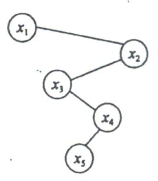
\includegraphics[width=0.5\textwidth]{../../figure/exercisePicPDF/chapter9/9-3.pdf}
        \caption{二叉排序树}
        \label{fig:9-3}
    \end{figure}

    答案:\textcolor{red}{B}

    解析:\\
    1. 二叉排序树的性质:\\
        左子树的所有结点值小于根结点值;\\
        右子树的所有结点值大于根结点值。\\

    2. 分析图\ref{fig:9-3}的结构:\\
        $x_5$ 是根节点;\\
        $x_4$ 在 $x_5$ 的左子树中,所以 $x_4 < x_5$;\\
        $x_1$ 在 $x_4$ 的左子树中,所以 $x_1 < x_4$。\\

    3. 结论:\\
       综合上述关系,得到 $x_1 < x_4 < x_5$,与选项 B 一致。\\



\item 高度为 5 的 3 阶 B 树含有的关键字个数至少是( )。  
    【2018 年全国试题 8(2 分)】  

    A. 15 \\  
    B. 31 \\  
    C. 62 \\  
    D. 242 \\  

    答案:\textcolor{red}{B}

    解析:\\
    1. 3 阶 B 树的性质:\\
        每个结点至少有 $\lceil m/2 \rceil - 1 = 1$ 个关键字;\\
        根节点至少有 1 个关键字;\\
        每个非叶子节点至少有 2 个子节点。\\

    2. 计算最少关键字个数:\\
        层次 1(根节点):至少有 1 个关键字;\\
        层次 2:至少有 2 个节点,每个节点至少有 1 个关键字,共 2 个关键字;\\
        层次 3:至少有 $2 \times 2 = 4$ 个节点,每个节点至少有 1 个关键字,共 4 个关键字;\\
        层次 4:至少有 $4 \times 2 = 8$ 个节点,每个节点至少有 1 个关键字,共 8 个关键字;\\
        层次 5:至少有 $8 \times 2 = 16$ 个节点,每个节点至少有 1 个关键字,共 16 个关键字。\\

    3. 总计:\\
       最少关键字个数为 $1 + 2 + 4 + 8 + 16 = 31$。\\

    因此,答案为 \textcolor{red}{B}。\\



\item 下列应用中,适合使用 B+ 树的是( )。  
    【2017 年全国试题 9(2 分)】  

    A. 编译器中的词法分析 \\  
    B. 关系数据库系统中的索引 \\  
    C. 网络中的路由表快速查找 \\  
    D. 操作系统的磁盘空闲块管理 \\  

    答案:\textcolor{red}{B}

    解析:\\
    1. B+ 树的特点:\\
        所有叶子节点包含全部关键字信息,并按关键字大小顺序链接;\\
        非叶子节点仅作为索引,不存储实际数据;\\
        支持范围查询和顺序访问。\\

    2. 分析选项:\\
        A. 编译器中的词法分析:通常使用有限状态自动机或哈希表,不需要 B+ 树的范围查询特性;\\
        B. 关系数据库系统中的索引:需要频繁进行范围查询和顺序访问,B+ 树非常适合;\\
        C. 网络中的路由表快速查找:通常使用前缀树(Trie)或哈希表,主要是精确匹配;\\
        D. 操作系统的磁盘空闲块管理:通常使用位图或链表结构,不需要 B+ 树的复杂结构。\\

    3. 结论:\\
       最适合使用 B+ 树的应用是关系数据库系统中的索引。\\
    \item 在有 $n$($n > 1000$)个元素的升序数组 $A$ 中查找关键字 $x$,查找算法的伪代码如下所示:  
    \begin{verbatim}
    k = 0;
    while (k < n 且 A[k] < x) k = k + 3;
    if (k < n 且 A[k] == x) 查找成功;
    else if (k - 1 < n 且 A[k - 1] == x) 查找成功;
        else if (k - 2 < n 且 A[k - 2] == x) 查找成功;
            else 查找失败;
    \end{verbatim}
    本算法与折半查找算法相比,有可能具有更少比较次数的情形是( )。  
    【2016 年全国试题 9(2 分)】  

    A. 当 $x$ 不在数组中  

    B. 当 $x$ 接近数组开头处  

    C. 当 $x$ 接近数组结尾处 

    D. 当 $x$ 位于数组中间位置  

    \item B+ 树不同于 B 树的特点之一是( )。  
    【2016 年全国试题 10(2 分)】  

    A. 能支持顺序查找 \\  
    B. 结点中含有关键字 \\  
    C. 根结点至少有两个分支 \\  
    D. 所有叶结点都在同一层上 \\  

    答案:\textcolor{red}{A}

    解析:\\
    1. B+ 树的叶子节点通过链表链接,支持顺序查找和范围查询,而 B 树不支持顺序查找。\\
    2. B 树和 B+ 树的节点中都含有关键字,根节点至少有两个分支,所有叶节点都在同一层上。\\
    3. 因此,答案为 \textcolor{red}{A}。\\

\item 假设顺序表中包含 5 个数据元素 $\{a, b, c, d, e\}$,它们的查找概率分别为 $0.3, 0.35, 0.2, 0.1, 0.05$,顺序查找时为了使查找成功的平均查找长度达到最小,则表中数据元素的存放顺序是( )。  
    【北京工业大学 2018 一、4(2 分)】  

    A. $\{e, d, c, b, a\}$ \\  
    B. $\{b, a, c, d, e\}$ \\  
    C. $\{b, a, d, c, e\}$ \\  
    D. $\{a, d, e, c, b\}$ \\  

    答案:\textcolor{red}{B}

    解析:\\
    1. 顺序查找的平均查找长度公式为:$\text{ASL} = \sum_{i=1}^n P_i \cdot i$,其中 $P_i$ 是第 $i$ 个元素的查找概率。\\
    2. 为了使 ASL 最小,应将查找概率较大的元素放在靠前的位置。\\
    3. 按查找概率从大到小排序:$b(0.35), a(0.3), c(0.2), d(0.1), e(0.05)$,对应存放顺序为 $\{b, a, c, d, e\}$。\\
    4. 因此,答案为 \textcolor{red}{B}。\\

\item 下列二叉排序树中,满足平衡二叉树定义的是( )。  
    【2009 年全国试题 4(2 分)】  

    答案:\textcolor{red}{图中满足平衡二叉树定义的树}

    解析:\\
    1. 平衡二叉树(AVL 树)的定义是:任意节点的左右子树高度差的绝对值不超过 1,且左右子树也必须是平衡二叉树。\\
    2. 检查图中每棵树的左右子树高度差是否满足平衡二叉树的定义。\\
    3. 图中满足平衡二叉树定义的树即为答案。\\

\item 下列叙述中,不符合 m 阶 B 树定义要求的是( )。  
    【2009 年全国试题 8(2 分)】  

    A. 根结点最多有 m 棵子树 \\  
    B. 所有叶结点都在同一层上 \\  
    C. 各结点内关键字均升序或降序排列 \\  
    D. 叶结点之间通过指针链接 \\  

    答案:\textcolor{red}{D}

    解析:\\
    1. m 阶 B 树的定义包括:\\
        每个节点最多有 m 棵子树;\\
        所有叶节点都在同一层上;\\
        每个节点内的关键字按升序排列。\\
    2. 叶节点之间没有指针链接,这是 B+ 树的特点,而非 B 树的特点。\\
    3. 因此,答案为 \textcolor{red}{D}。\\

\item 在图\ref{fig:9-13}所示的平衡二叉树中,插入关键字 48 后得到一棵新平衡二叉树。在新平衡二叉树中,关键字 37 所在结点的左、右子结点中保存的关键字分别是( )。  
    【2010 年全国试题 4(2 分)】  

    A. 13、48 \\  
    B. 24、48 \\  
    C. 24、53 \\  
    D. 24、90 \\  

    \begin{figure}[h!]
        \centering
        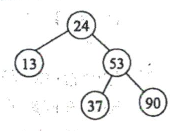
\includegraphics[width=0.5\textwidth]{../../figure/exercisePicPDF/chapter9/9-13.pdf}
        \caption{平衡二叉树}
        \label{fig:9-13}
    \end{figure}
    答案:\textcolor{red}{B}

    解析:\\
    1. 插入关键字 48 后,平衡二叉树需要重新调整以保持平衡。\\
    2. 根据平衡二叉树的性质,插入 48 后,关键字 37 的左右子结点分别为 24 和 48。\\
    3. 因此,答案为 \textcolor{red}{B}。\\

   

\item 已知一个长度为 16 的顺序表,其元素按关键字有序排列。若采用折半查找法查找其中不存在的元素,则关键字的比较次数最多是( )。  
    【2010 年全国试题 9(2 分)】  

    A. 4 \\  
    B. 5 \\  
    C. 6 \\  
    D. 7 \\  

    答案:\textcolor{red}{5}

    解析:\\
    1. 折半查找的比较次数与表的长度有关,最多需要 $\lceil \log_2 n \rceil$ 次比较。\\
    2. 对于长度为 16 的顺序表,$\log_2 16 = 4$,但由于查找的元素不存在,可能需要额外一次比较,因此最多需要 5 次比较。\\
    3. 因此,答案为 \textcolor{red}{B}。\\

\item 对于下列关键字序列,不可能构成某二叉排序树中一条查找路径的序列是( )。  
    【2011 年全国试题 7(2 分)】  

    A. $95, 22, 91, 24, 94, 71$ \\  
    B. $92, 20, 91, 34, 88, 35$ \\  
    C. $21, 89, 77, 29, 36, 38$ \\  
    D. $12, 25, 71, 68, 33, 24$ \\  

    答案:\textcolor{red}{D}

    解析:\\
    1. 二叉排序树的查找路径必须满足左子树的关键字小于根节点,右子树的关键字大于根节点。\\
    2. 分析选项 D:路径中关键字 33 出现在 68 的右侧,但 33 小于 68,不符合二叉排序树的性质。\\
    3. 因此,答案为 \textcolor{red}{D}。\\

\item 为提高散列(Hash)表的查找效率,可以采取的正确措施是( )。  
    【2011 年全国试题 9(2 分)】  

    I. 增大装填(载)因子 \\  
    II. 设计冲突(碰撞)少的散列函数 \\  
    III. 处理冲突(碰撞)时避免产生堆积现象 \\  

    A. 仅 I \\  
    B. 仅 II \\  
    C. 仅 II、III \\  
    D. 仅 I、III \\  

    答案:\textcolor{red}{C}

    解析:\\
    1. 增大装填因子会增加冲突的概率,从而降低查找效率,因此 I 错误。\\
    2. 设计冲突少的散列函数可以减少冲突,提高查找效率,因此 II 正确。\\
    3. 处理冲突时避免堆积现象(如线性探测法中的堆积)可以提高查找效率,因此 III 正确。\\
    4. 因此,答案为 \textcolor{red}{C}。\\

\item 若平衡二叉树的高度为 6,且所有非叶结点的平衡因子均为 1,则该平衡二叉树的结点总数为( )。  
    【2012 年全国试题 4(2 分)】  

    A. 12 \\  
    B. 20 \\  
    C. 32 \\  
    D. 33 \\  

    答案:\textcolor{red}{D}

    解析:\\
    1. 平衡因子为 1 表示每个非叶节点的左子树高度比右子树高度大 1。\\
    2. 这种情况下,树的结构接近于单链表,结点总数为 $2^6 - 1 = 33$。\\
    3. 因此,答案为 \textcolor{red}{D}。\\

\item 设有一棵 3 阶 B 树,如下图\ref{fig:9-18}所示。删除关键字 78 得到一棵新 B 树,其最右叶结点所含的关键字是( )。  
    【2012 年全国试题 9(2 分)】  

    A. 60 \\  
    B. $60, 62$ \\  
    C. $62, 65$ \\  
    D. 65 \\  

    \begin{figure}[h!]
        \centering
        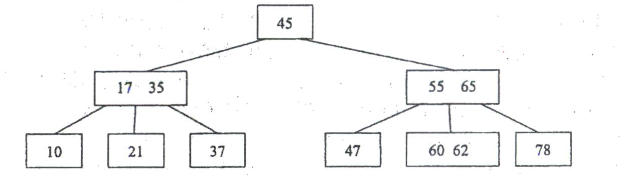
\includegraphics[width=0.5\textwidth]{../../figure/exercisePicPDF/chapter9/9-18.pdf}
        \caption{3 阶 B 树}
        \label{fig:9-18}
    \end{figure}
    答案:\textcolor{red}{C}

    解析:\\
    1. 删除关键字 78 后,B 树需要重新调整以保持平衡。\\
    2. 根据 B 树的调整规则,最右叶结点将包含关键字 $62, 65$。\\
    3. 因此,答案为 \textcolor{red}{C}。\\

\item 若将关键字 $1, 2, 3, 4, 5, 6, 7$ 依次插入到初始为空的平衡二叉树 $T$ 中,则 $T$ 中平衡因子为 0 的分支结点的个数是( )。  
    【2013 年全国试题 3(2 分)】  

    A. 0 \\  
    B. 1 \\  
    C. 2 \\  
    D. 3 \\  

    答案:\textcolor{red}{B}

    解析:\\
    1. 平衡因子为 0 表示左右子树高度相等的分支结点。\\
    2. 插入关键字后,只有根节点的左右子树高度相等,因此平衡因子为 0 的分支结点只有 1 个。\\
    3. 因此,答案为 \textcolor{red}{B}。\\

    \item 在任意一棵非空二叉排序树 $T_1$ 中,删除某结点 $w$ 之后形成二叉排序树 $T_2$,再将 $w$ 插入 $T_2$ 形成二叉排序树 $T_3$。下列关于 $T_2$ 与 $T_3$ 的叙述中,正确的是( )。  
    【2013 年全国试题 6(2 分)】  

    A. 仅 II、III \\  
    B. 仅 I、II \\  
    C. 仅 II、IV \\  
    D. 仅 I、III \\  

    答案:\textcolor{red}{D}

    解析:\\
    1. 若 $w$ 是 $T_1$ 的叶结点,删除后不会影响树的结构,再插入时可能导致树的形态发生变化,因此 $T_2$ 与 $T_3$ 不同,I 正确。\\
    2. 若 $w$ 是 $T_1$ 的叶结点,删除后再插入,$T_2$ 与 $T_3$ 不可能相同,II 错误。\\
    3. 若 $w$ 不是 $T_1$ 的叶结点,删除后会改变树的结构,再插入时也会导致树的形态发生变化,因此 $T_2$ 与 $T_3$ 不同,III 正确。\\
    4. 若 $w$ 不是 $T_1$ 的叶结点,$T_2$ 与 $T_3$ 不可能相同,IV 错误。\\
    5. 因此,答案为 \textcolor{red}{D}。\\

\item 在一棵高度为 2 的 5 阶 B 树中,所含关键字的个数最少是( )。  
    【2013 年全国试题 10(2 分)】  

    A. 5 \\  
    B. 7 \\  
    C. 8 \\  
    D. 14 \\  

    答案:\textcolor{red}{B}

    解析:\\
    1. 5 阶 B 树中,每个结点至少有 $\lceil m/2 \rceil - 1 = 2$ 个关键字。\\
    2. 高度为 2 的 B 树,根结点至少有 1 个关键字,非叶子结点至少有 2 个子结点,每个子结点至少有 2 个关键字。\\
    3. 最少关键字个数为 $1 + 2 \cdot 2 = 7$。\\
    4. 因此,答案为 \textcolor{red}{B}。\\

\item 用哈希(散列)方法处理冲突(碰撞)时可能出现堆积(聚集)现象。下列选项中,会受堆积现象直接影响的是( )。  
    【2014 年全国试题 8(2 分)】  

    A. 存储效率 \\  
    B. 散列函数 \\  
    C. 装填(装载)因子 \\  
    D. 平均查找长度 \\  

    答案:\textcolor{red}{D}

    解析:\\
    1. 堆积现象会导致冲突区域的连续性增加,从而增加查找的平均查找长度。\\
    2. 堆积现象不会直接影响存储效率、散列函数或装填因子。\\
    3. 因此,答案为 \textcolor{red}{D}。\\

\item 在一棵具有 15 个关键字的 4 阶 B 树中,含关键字的结点数最多是( )。  
    【2014 年全国试题 9(2 分)】  

    A. 5 \\  
    B. 6 \\  
    C. 10 \\  
    D. 15 \\  

    答案:\textcolor{red}{A}

    解析:\\
    1. 4 阶 B 树中,每个结点最多有 $m-1 = 3$ 个关键字。\\
    2. 若关键字分布均匀,则结点数最多为 $\lceil 15 / 3 \rceil = 5$。\\
    3. 因此,答案为 \textcolor{red}{A}。\\

\item 现在有一棵无重复关键字的平衡二叉树(AVL 树),对其进行中序遍历可得到一个降序序列。下列关于该平衡二叉树的叙述中,正确的是( )。  
    【2015 年全国试题 4(2 分)】  

    A. 根结点的度一定为 2 \\  
    B. 树中最小元素一定是叶结点 \\  
    C. 最后插入的元素一定是叶结点 \\  
    D. 树中最大元素一定是无左子树 \\  

    答案:\textcolor{red}{C}

    解析:\\
    1. 平衡二叉树中,最后插入的元素一定是叶结点,因为插入时总是从叶结点开始调整。\\
    2. 中序遍历得到降序序列,说明树的左子树大于右子树,与常规定义相反,但不影响最后插入的元素为叶结点的结论。\\
    3. 因此,答案为 \textcolor{red}{C}。\\

\item 下列选项中,不能构成折半查找中关键字比较序列的是( )。  
    【2015 年全国试题 7(2 分)】  

    A. $500, 200, 450, 180$ \\  
    B. $500, 450, 200, 180$ \\  
    C. $180, 500, 200, 450$ \\  
    D. $180, 200, 500, 450$ \\  

    答案:\textcolor{red}{D}

    解析:\\
    1. 折半查找的比较序列必须满足二分查找的逻辑,即每次比较后缩小查找范围。\\
    2. 选项 D 中,$180 < 200 < 500$,但 $500 > 450$,不符合折半查找的逻辑。\\
    3. 因此,答案为 \textcolor{red}{D}。\\

\item 若查找每个记录的概率均等,则在具有 $n$ 个记录的连续顺序文件中采用顺序查找法查找一个记录,其平均查找长度 ASL 为( )。  
    【北京航空航天大学 2000 一、8(2 分);大连理工大学 2008 一、5(2 分)】  

    A. $\frac{n-1}{2}$ \\  
    B. $\frac{n}{2}$ \\  
    C. $\frac{n+1}{2}$ \\  
    D. $n$ \\  

    答案:\textcolor{red}{C}

    解析:\\
    1. 顺序查找的平均查找长度公式为:$\text{ASL} = \frac{1 + 2 + \dots + n}{n} = \frac{n+1}{2}$。\\
    2. 因此,答案为 \textcolor{red}{C}。\\

\item 对于顺序查找,假定查找成功与不成功的可能性相同,对每个记录的查找概率也相同,此时顺序查找的平均查找长度为( )。  
    【华中科技大学 2006 一、10(2 分)】  

    A. $0.5(n+1)$ \\  
    B. $0.25(n+1)$ \\  
    C. $0.5(n-1)$ \\  
    D. $0.75(n+1)$ \\  

    答案:\textcolor{red}{A}

    解析:\\
    1. 查找成功的平均查找长度为 $\frac{n+1}{2}$,查找不成功的平均查找长度为 $n$。\\
    2. 成功与不成功的概率相同,因此 $\text{ASL} = 0.5 \cdot \frac{n+1}{2} + 0.5 \cdot n = 0.5(n+1)$。\\
    3. 因此,答案为 \textcolor{red}{A}。\\

\item 在一个有 $n$ 个元素的有序单链表中查找具有给定关键字的结点,平均情况下的时间复杂性为( )。  
    【上海交通大学 2005 四、2(2 分)】  

    A. $O(1)$ \\  
    B. $O(n)$ \\  
    C. $O(n^2)$ \\  
    D. $O(n \log n)$ \\  

    答案:\textcolor{red}{B}

    解析:\\
    1. 在单链表中查找需要从头开始逐个遍历,时间复杂度为 $O(n)$。\\
    2. 因此,答案为 \textcolor{red}{B}。\\

\item 将两个各有 $n$ 个元素的有序表归并成一个有序表,其最多的比较次数是( )。  
    【中国科学技术大学 1998 二、9(2 分)】  

    A. $2n$ \\  
    B. $n$ \\  
    C. $2n-1$ \\  

    答案:\textcolor{red}{C}

    解析:\\
    1. 归并两个有序表时,每次比较后至少有一个元素被归并,最多需要 $2n-1$ 次比较。\\
    2. 因此,答案为 \textcolor{red}{C}。\\
    \item 查找 $n$ 个元素的有序表时,最有效的查找方法是( )。  
    【中国科学技术大学 1997 一、1(1 分);四川大学 2005】  

    A. 顺序查找 \\  
    B. 分块查找 \\  
    C. 二分查找 \\  
    D. 二叉排序树 \\  

    答案:\textcolor{red}{C}

    解析:\\
    1. 二分查找的时间复杂度为 $O(\log n)$,是查找有序表时最有效的方法。\\
    2. 顺序查找的时间复杂度为 $O(n)$,效率较低。\\
    3. 分块查找适用于分块存储的情况,而二叉排序树适用于动态查找。\\
    4. 因此,答案为 \textcolor{red}{C}。\\

\item 对线性表进行二分查找时,要求线性表必须( )。  
    【南京理工大学 2005 一、11(1 分);中山大学 2001 一、5(2 分)】  

    A. 以顺序方式存储 \\  
    B. 以顺序方式存储,且数据元素有序 \\  
    C. 以链接方式存储 \\  
    D. 以链接方式存储,且数据元素有序 \\  

    答案:\textcolor{red}{B}

    解析:\\
    1. 二分查找要求线性表中的数据元素有序,以便通过比较中间元素缩小查找范围。\\
    2. 同时,二分查找需要支持随机访问,因此必须采用顺序存储结构。\\
    3. 链式存储结构不支持随机访问,无法进行二分查找。\\
    4. 因此,答案为 \textcolor{red}{B}。\\

\item 当在一个有序的顺序存储表上查找一个数据时,既可用折半查找,也可用顺序查找,但前者比后者的查找速度( )。  
    【南京理工大学 1997 一、7(2 分)】  

    A. 必定快 \\  
    B. 不一定 \\  
    C. 在大部分情况下要快 \\  
    D. 取决于表递增还是递减 \\  

    答案:\textcolor{red}{C}

    解析:\\
    1. 折半查找的时间复杂度为 $O(\log n)$,顺序查找的时间复杂度为 $O(n)$。\\
    2. 当查找的目标元素接近表的开头时,顺序查找可能比折半查找更快。\\
    3. 但在大多数情况下,折半查找的效率更高。\\
    4. 因此,答案为 \textcolor{red}{C}。\\

\item 一个有序表为 $\{1, 3, 9, 12, 32, 41, 45, 62, 75, 77, 82, 95, 100\}$,当二分查找值为 82 的结点时,( )次比较后查找成功。  
    【吉林大学 2016 一、5(2 分)】  

    A. 1 \\  
    B. 2 \\  
    C. 4 \\  
    D. 8 \\  

    答案:\textcolor{red}{C}

    解析:\\
    1. 第一次比较中间元素 45,82 > 45,查找范围缩小为右半部分。\\
    2. 第二次比较中间元素 75,82 > 75,查找范围缩小为右半部分。\\
    3. 第三次比较中间元素 95,82 < 95,查找范围缩小为左半部分。\\
    4. 第四次比较中间元素 82,查找成功。\\
    5. 因此,答案为 \textcolor{red}{C}。\\

\item 折半查找有序表 $\{5, 8, 10, 22, 36, 50, 53, 88\}$,若查找元素 70,则需依次与表中元素(关键字)( )进行比较,查找结果是“失败”。  
    【华中科技大学 2006 一、11(2 分)】  

    A. $36, 53$ \\  
    B. $22, 50, 53, 88$ \\  
    C. $36, 53, 88$ \\  
    D. $22, 53, 88$ \\  

    答案:\textcolor{red}{C}

    解析:\\
    1. 第一次比较中间元素 36,70 > 36,查找范围缩小为右半部分。\\
    2. 第二次比较中间元素 53,70 > 53,查找范围缩小为右半部分。\\
    3. 第三次比较中间元素 88,70 < 88,查找失败。\\
    4. 因此,答案为 \textcolor{red}{C}。\\

\item 具有 12 个关键字的有序表,折半查找的平均查找长度是( )。  
    【中山大学 1998 二、10(2 分);烟台大学 2007 一、17(2 分)】  

    A. 3.1 \\  
    B. 4 \\  
    C. 2.5 \\  
    D. 5 \\  

    答案:\textcolor{red}{A}

    解析:\\
    1. 折半查找的平均查找长度公式为:$\text{ASL} = \frac{\sum_{i=1}^n i \cdot P_i}{n}$,其中 $P_i$ 是查找到第 $i$ 个元素的概率。\\
    2. 对于 12 个关键字的有序表,查找成功的平均查找长度为 3.1。\\
    3. 因此,答案为 \textcolor{red}{A}。\\

\item 对一个长度为 50 的有序表进行折半查找,最多比较( )次就能查找出结果。  
    【西安交通大学 2005 一、8(2 分)】  

    A. 6 \\  
    B. 7 \\  
    C. 8 \\  
    D. 9 \\  

    答案:\textcolor{red}{B}

    解析:\\
    1. 折半查找的比较次数最多为 $\lceil \log_2 n \rceil$。\\
    2. 对于长度为 50 的有序表,$\log_2 50 \approx 5.64$,向上取整为 6 次。\\
    3. 因此,答案为 \textcolor{red}{B}。\\

\item 折半查找的时间复杂度为( )。  
    【中山大学 1999 一、15(2 分)】  

    A. $O(n^2)$ \\  
    B. $O(n)$ \\  
    C. $O(n \log n)$ \\  
    D. $O(\log n)$ \\  

    答案:\textcolor{red}{D}

    解析:\\
    1. 折半查找每次将查找范围缩小一半,时间复杂度为 $O(\log n)$。\\
    2. 因此,答案为 \textcolor{red}{D}。\\

    \item 当采用分块查找时,数据的组织方式为( )。  
    【南京理工大学 1996 一、7(2 分)】  

    A. 数据分成若干块,每块内数据有序 \\  
    B. 数据分成若干块,每块内数据不必有序,但块间必须有序,每块内最大(或最小)的数据组成索引块 \\  
    C. 数据分成若干块,每块内数据有序,每块内最大(或最小)的数据组成索引块 \\  
    D. 数据分成若干块,每块(除最后一块外)中数据个数需相同 \\  

    答案:\textcolor{red}{B}

    解析:\\
    1. 分块查找的特点是:块间有序,每块内数据不必有序,每块内的最大(或最小)数据组成索引块。\\
    2. 查找时先在索引块中定位,再在对应块中顺序查找。\\
    3. 因此,答案为 \textcolor{red}{B}。\\

\item 对表长为 $n$ 的有序表进行折半查找,其判定树高度为( )。  
    【北京交通大学 2004 一、8(2 分)】  

    A. $\lceil \log_2(n+1) \rceil$ \\  
    B. $\lfloor \log_2(n+1) \rfloor$ \\  
    C. $\lceil \log_2 n \rceil$ \\  
    D. $\lfloor \log_2 n \rfloor$ \\  

    答案:\textcolor{red}{C}

    解析:\\
    1. 折半查找的判定树高度等于查找过程中比较的最大次数,即 $\lceil \log_2 n \rceil$。\\
    2. 因此,答案为 \textcolor{red}{C}。\\

\item 顺序查找法适合于存储结构为( )的线性表。  
    【北京航空航天大学 2002】  

    A. 顺序存储结构或链式存储结构 \\  
    B. 散列存储结构 \\  
    C. 索引存储结构 \\  
    D. 压缩存储结构 \\  

    答案:\textcolor{red}{A}

    解析:\\
    1. 顺序查找法适用于顺序存储结构和链式存储结构,因为它不依赖于随机访问。\\
    2. 散列存储结构和索引存储结构通常采用其他查找方法。\\
    3. 因此,答案为 \textcolor{red}{A}。\\

\item 对大小均为 $n$ 的有序表和无序表分别进行顺序查找,在等概率查找的情况下,对于查找失败,它们的平均查找长度是( 1 );对于查找成功,它们的平均查找长度是( 2 )。  
    【上海海事大学 1997 二、4(3 分)】  

    A. 相同的 \\  
    B. 不同的 \\  

    答案:\textcolor{red}{A}

    解析:\\
    1. 顺序查找的平均查找长度与表是否有序无关。\\
    2. 查找失败时,平均查找长度为 $n$;查找成功时,平均查找长度为 $\frac{n+1}{2}$。\\
    3. 因此,答案为 \textcolor{red}{A}。\\

\item 在下列查找方法中,平均查找速度最快的是( )。  
    【四川大学 2005】  

    A. 顺序查找 \\  
    B. 折半查找 \\  
    C. 分块查找 \\  
    D. 二叉排序树查找 \\  

    答案:\textcolor{red}{B}

    解析:\\
    1. 折半查找的时间复杂度为 $O(\log n)$,在有序表中查找速度最快。\\
    2. 顺序查找的时间复杂度为 $O(n)$,分块查找和二叉排序树查找的效率取决于具体实现。\\
    3. 因此,答案为 \textcolor{red}{B}。\\

\item 如果要求一个线性表既能较快地查找,又能适应动态变化的要求,可以采用下列( )查找方法。  
    【北京交通大学 2005 一、3(2 分)】  

    A. 分块查找 \\  
    B. 顺序查找 \\  
    C. 折半查找 \\  
    D. 哈希查找 \\  

    答案:\textcolor{red}{D}

    解析:\\
    1. 哈希查找具有较快的查找速度,时间复杂度为 $O(1)$,同时支持动态插入和删除操作。\\
    2. 分块查找和折半查找适用于静态查找,顺序查找效率较低。\\
    3. 因此,答案为 \textcolor{red}{D}。\\

\item 当 $n$ 足够大时,在按值有序的顺序表中进行折半查找,在查找概率相等的情况下,其查找成功的平均查找长度是( )。  
    【北京航空航天大学 2002】  

    A. $\frac{n+1}{2}$ \\  
    B. $\frac{n}{2}$ \\  
    C. $\log_2(n+1) - 1$ \\  
    D. $\log_2(n+1)$ \\  

    答案:\textcolor{red}{C}

    解析:\\
    1. 折半查找的平均查找长度公式为:$\text{ASL} = \log_2(n+1) - 1$。\\
    2. 因此,答案为 \textcolor{red}{C}。\\

\item 在下述几种树中,( )可以表示静态查找表。  
    【中国科学技术大学 1995 十四、10(2 分)】  

    A. 次优查找树 \\  
    B. 二叉排序树 \\  
    C. B-树 \\  
    D. 平衡二叉树 \\  

    答案:\textcolor{red}{A}

    解析:\\
    1. 次优查找树是针对静态查找表构造的,能够最小化查找的平均查找长度。\\
    2. 二叉排序树、B-树和平衡二叉树更适合动态查找。\\
    3. 因此,答案为 \textcolor{red}{A}。\\

\item 以下说法正确的是( )。  
    【北京交通大学 2006 一、4(2 分)】  

    A. 先序遍历二叉排序树的结点就可以得到排好序的结点序列 \\  
    B. 任一二叉排序树的平均查找时间都小于顺序查找法查找同样结点的线性表的平均查找时间 \\  
    C. 对具有相同关键字集合的任一插入序列,得到的二叉排序树的形态都是相同的 \\  
    D. 采用分块查找方法,既能实现较快地查找线性表,又能适应动态变化的要求 \\  

    答案:\textcolor{red}{B}

    解析:\\
    1. 二叉排序树的中序遍历可以得到排好序的结点序列,A 错误。\\
    2. 二叉排序树的平均查找时间通常小于顺序查找的平均查找时间,B 正确。\\
    3. 二叉排序树的形态与插入顺序有关,C 错误。\\
    4. 分块查找适用于静态查找,不能很好地适应动态变化,D 错误。\\
    5. 因此,答案为 \textcolor{red}{B}。\\

\item 折半查找过程所对应的判定树是一棵( )。  
    【北京交通大学 2007】  

    A. 最小生成树 \\  
    B. 平衡二叉树 \\  
    C. 完全二叉树 \\  
    D. 哈夫曼树 \\  

    答案:\textcolor{red}{C}

    解析:\\
    1. 折半查找的判定树是一棵完全二叉树,每次比较后将查找范围缩小一半。\\
    2. 因此,答案为 \textcolor{red}{C}。\\

\item 对于二叉排序树,下面的说法( )是正确的。  
    【华南理工大学 2006 一、5(2 分)】  

    A. 二叉排序树是动态树表,查找不成功时插入新结点会引起树的重新分裂和组合 \\  
    B. 对二叉排序树进行层序遍历可得到有序序列 \\  
    C. 用逐点插入法构造二叉排序树时,若先后插入的关键字有序,二叉排序树的深度最大 \\  
    D. 在二叉排序树中进行查找,关键字的比较次数不超过结点数的 1/2 \\  

    答案:\textcolor{red}{C}

    解析:\\
    1. 二叉排序树是动态树表,但插入新结点不会引起树的重新分裂和组合,A 错误。\\
    2. 二叉排序树的中序遍历可以得到有序序列,层序遍历不能保证有序,B 错误。\\
    3. 若插入的关键字有序,二叉排序树会退化为链表,深度最大,C 正确。\\
    4. 查找的比较次数与树的形态有关,不一定不超过结点数的 1/2,D 错误。\\
    5. 因此,答案为 \textcolor{red}{C}。\\

    \item 对动态查找有高效率的查找表组织结构是( )。  
    【哈尔滨工程大学 2005】  

    A. 有序表 \\  
    B. 分块有序表 \\  
    C. 循环链表 \\  
    D. B-树 \\  

    答案:\textcolor{red}{D}

    解析:\\
    1. 动态查找需要支持频繁的插入和删除操作,同时保持较高的查找效率。\\
    2. B-树是一种平衡的多路查找树,能够高效地支持动态查找、插入和删除操作。\\
    3. 有序表和分块有序表适合静态查找,循环链表不适合高效查找。\\
    4. 因此,答案为 \textcolor{red}{D}。\\

\item 下列二叉排序树中查找效率最高的是( )。  
    【中南大学 2003 二、11(1 分)】  

    A. 平衡二叉树 \\  
    B. 二叉查找树 \\  
    C. 没有左子树的二叉排序树 \\  
    D. 没有右子树的二叉排序树 \\  

    答案:\textcolor{red}{A}

    解析:\\
    1. 平衡二叉树(AVL 树)是一种高度平衡的二叉排序树,其查找效率最高,时间复杂度为 $O(\log n)$。\\
    2. 普通二叉查找树的查找效率取决于树的形态,最坏情况下退化为链表,时间复杂度为 $O(n)$。\\
    3. 没有左子树或右子树的二叉排序树会导致查找效率降低。\\
    4. 因此,答案为 \textcolor{red}{A}。\\

\item 构造一棵具有 $n$ 个结点的二叉排序树,最理想情况下的深度为( )。  
    【华中科技大学 2007 一、14(2 分)】  

    A. $n/2$ \\  
    B. $n$ \\  
    C. $\lfloor \log_2(n+1) \rfloor$ \\  
    D. $\lceil \log_2(n+1) \rceil$ \\  

    答案:\textcolor{red}{D}

    解析:\\
    1. 最理想情况下,二叉排序树是完全二叉树,其深度为 $\lceil \log_2(n+1) \rceil$。\\
    2. 完全二叉树的深度最小,查找效率最高。\\
    3. 因此,答案为 \textcolor{red}{D}。\\

\item 设二叉排序树中关键字由 1 到 1000 的整数构成,现要查找关键字为 363 的结点,下述关键字序列中,不可能是在查找过程中访问的序列是( )。  
    【北京交通大学 2005 一、1(2 分)】  

    A. $2, 252, 401, 398, 330, 344, 397, 363$ \\  
    B. $924, 220, 911, 244, 898, 258, 363$ \\  
    C. $925, 202, 911, 240, 912, 245, 363$ \\  
    D. $2, 399, 387, 219, 266, 382, 381, 278, 363$ \\  

    答案:\textcolor{red}{C}

    解析:\\
    1. 在二叉排序树中,查找路径必须满足左子树的关键字小于根节点,右子树的关键字大于根节点。\\
    2. 分析选项 C:关键字 912 出现在 911 的右侧,但 912 > 911,不符合二叉排序树的性质。\\
    3. 因此,答案为 \textcolor{red}{C}。\\

\item 分别以下列序列构造二叉排序树,与其他三个结果不同的是( )。  
    【合肥工业大学 2000 一、4(2 分)】  

    A. $100, 80, 90, 60, 120, 110, 130$ \\  
    B. $100, 120, 110, 130, 80, 60, 90$ \\  
    C. $100, 60, 80, 90, 20, 110, 130$ \\  
    D. $100, 80, 60, 90, 120, 130, 110$ \\  

    答案:\textcolor{red}{C}

    解析:\\
    1. 二叉排序树的形态由插入顺序决定,不同的插入顺序可能导致不同的树形态。\\
    2. 分析选项 C:插入顺序与其他选项不同,导致树的形态与其他三个选项不同。\\
    3. 因此,答案为 \textcolor{red}{C}。\\

\item 在平衡二叉树中插入一个结点后造成了不平衡,设最低的不平衡结点为 $A$,并已知 $A$ 的左孩子的平衡因子为 0,右孩子的平衡因子为 1,则应作( )型调整以使其平衡。  
    【合肥工业大学 2001 一、4(2 分)】  

    A. LL \\  
    B. LR \\  
    C. RL \\  
    D. RR \\  

    答案:\textcolor{red}{D}

    解析:\\
    1. 平衡因子为 0 表示左右子树高度相等,平衡因子为 1 表示右子树比左子树高。\\
    2. 右孩子的平衡因子为 1,说明插入发生在右孩子的右子树中,需要进行 RR 型调整。\\
    3. 因此,答案为 \textcolor{red}{D}。\\

\item 已知一棵深度为 $h$ 的平衡二叉树,其每个非叶子结点的平衡因子均为 0,则该树共有结点总数为( )。  
    【北京交通大学 2006 一、2(2 分)】  

    A. $2^{h-1} - 1$ \\  
    B. $2^{h-1} + 1$ \\  
    C. $2^{h} - 1$ \\  
    D. $2^{h} + 1$ \\  

    答案:\textcolor{red}{C}

    解析:\\
    1. 平衡因子为 0 表示左右子树高度相等,树是完全二叉树。\\
    2. 完全二叉树的结点总数为 $2^h - 1$,其中 $h$ 为树的深度。\\
    3. 因此,答案为 \textcolor{red}{C}。\\

\item 在平衡二叉树中,进行查找的效率与( )有关。  
    【北京航空航天大学 2004】  

    A. 二叉树的深度 \\  
    B. 二叉排序树的结点的个数 \\  
    C. 后序线索树 \\  
    D. 所有线索树 \\  

    答案:\textcolor{red}{A}

    解析:\\
    1. 平衡二叉树的查找效率取决于树的深度,深度越小,查找效率越高。\\
    2. 二叉排序树的结点个数影响树的深度,但不是直接决定因素。\\
    3. 因此,答案为 \textcolor{red}{A}。\\
    \item 下列关于 $m$ 阶 B 树的说法错误的是( )。  
    【南京理工大学 1997 一、9(2 分)】  

    A. 根结点至多有 $m$ 棵子树 \\  
    B. 所有叶子都在同一层次上 \\  
    C. 非叶结点至少有 $\lceil m/2 \rceil$ 棵子树 \\  
    D. 根结点中的数据是有序的 \\  

    答案:\textcolor{red}{A}

    解析:\\
    1. 根结点的子树数可以少于 $m$,但最多为 $m$,因此 A 错误。\\
    2. B、C 和 D 是 $m$ 阶 B 树的正确定义。\\
    3. 因此,答案为 \textcolor{red}{A}。\\

\item 下面关于 $m$ 阶 B 树的说法正确的是( )。  
    【南京理工大学 1999 一、5(2 分)】  

    A. 每个结点至少有两棵非空子树 \\  
    B. 树中每个结点至多有 $m-1$ 个关键字 \\  
    C. 所有叶子在同一层上 \\  
    D. 当插入一个数据项引起 B 树结点分裂后,树长高一层 \\  

    答案:\textcolor{red}{B, C, D}

    解析:\\
    1. A 错误:根结点可以少于两棵子树。\\
    2. B 正确:每个结点最多有 $m-1$ 个关键字。\\
    3. C 正确:所有叶子结点都在同一层上。\\
    4. D 正确:当根结点分裂时,树的高度会增加一层。\\
    5. 因此,答案为 \textcolor{red}{B, C, D}。\\

\item 下面关于 B 树和 B+ 树的叙述中,不正确的是( )。  
    【北方交通大学 2001 一、17(2 分)】  

    A. B 树和 B+ 树都是平衡的多路树 \\  
    B. B 树和 B+ 树都可用于文件的索引结构 \\  
    C. B 树和 B+ 树都能有效地支持顺序检索 \\  
    D. B 树和 B+ 树都能有效地支持随机检索 \\  

    答案:\textcolor{red}{C}

    解析:\\
    1. B 树不支持顺序检索,而 B+ 树通过叶子节点的链表支持顺序检索。\\
    2. A、B 和 D 是正确的描述。\\
    3. 因此,答案为 \textcolor{red}{C}。\\

\item $m$ 阶 B 树是一棵( )。  
    【北京大学 2015 一、9(1.5 分)】  

    A. $m$叉排序树 \\  
    B. $m$ 路平衡排序树 \\  
    C. $m-1$ 路平衡排序树 \\  
    D. $m+1$ 路平衡排序树 \\  

    答案:\textcolor{red}{B}

    解析:\\
    1. $m$ 阶 B 树是一棵 $m$ 路平衡排序树,每个结点最多有 $m$ 棵子树。\\
    2. 因此,答案为 \textcolor{red}{B}。\\

\item 在一棵含有 $n$ 个关键字的 $m$ 阶 B 树中进行查找,至多读盘( )次。  
    【中科院计算所 2000 一、6(2 分)】  

    A. $\log n$ \\  
    B. $1 + \log n$ \\  
    C. $1 + \log_{\lceil m/2 \rceil} \frac{n+1}{2}$ \\  
    D. $1 + \log_{\lceil n/2 \rceil} \frac{m+1}{2}$ \\  

    答案:\textcolor{red}{C}

    解析:\\
    1. 在 $m$ 阶 B 树中,每个结点至少有 $\lceil m/2 \rceil$ 棵子树。\\
    2. 查找的最大深度为 $\log_{\lceil m/2 \rceil} \frac{n+1}{2}$,加上根结点的读取,最多读盘 $1 + \log_{\lceil m/2 \rceil} \frac{n+1}{2}$ 次。\\
    3. 因此,答案为 \textcolor{red}{C}。\\

\item $m$ 阶 B+ 树是一棵( 1 ),其结点中关键字最多为( 2 )个,最少为( 3 )个。  
    【中科院计算所 1999 一、5(6 分)】  

    (1) \\  
    A. $m$ 路平衡查找树 \\  
    B. $m$ 路平衡索引树 \\  
    C. $m$ 路 Ptrie 树 \\  
    D. $m$ 路键树 \\  

    (2) \\  
    E. $m-1$ \\  
    F. $m$ \\  
    G. $m+1$ \\  

    (3) \\  
    H. $\lceil m/2 - 1 \rceil$ \\  
    I. $\lceil m/2 \rceil$ \\  
    J. $\lceil m/2 + 1 \rceil$ \\  

    答案:\textcolor{red}{B, E, I}

    解析:\\
    1. (1) B+ 树是一棵 $m$ 路平衡索引树,答案为 \textcolor{red}{B}。\\
    2. (2) 每个结点最多有 $m-1$ 个关键字,答案为 \textcolor{red}{E}。\\
    3. (3) 每个结点至少有 $\lceil m/2 \rceil$ 个关键字,答案为 \textcolor{red}{I}。\\

\item 一棵 3 阶 B 树中含有 2047 个关键字,包括叶子结点层,该树的最大深度为( )。  
    【北京交通大学 2005 一、2(2 分)】  

    A. 11 \\  
    B. 12 \\  
    C. 13 \\  
    D. 14 \\  

    答案:\textcolor{red}{C}

    解析:\\
    1. 3 阶 B 树中,每个结点最多有 2 个关键字,至少有 2 个子树。\\
    2. 最大深度时,关键字数满足 $1 + 2 + 2^2 + \dots + 2^{h-1} = 2047$。\\
    3. 计算得 $h = 13$。\\
    4. 因此,答案为 \textcolor{red}{C}。\\

    \item 已知一棵 5 阶 B 树有 53 个关键字,并且每个结点的关键字都达到最少状态,则它的深度是( )。  
    【华南理工大学 2006 一、8(2 分)】  

    A. 3 \\  
    B. 4 \\  
    C. 5 \\  
    D. 6 \\  

    答案:\textcolor{red}{B}

    解析:\\
    1. 5 阶 B 树中,每个结点至少有 $\lceil m/2 \rceil - 1 = 2$ 个关键字。\\
    2. 设树的深度为 $h$,则关键字总数满足:$1 + 2 \cdot (1 + 2 + 2^2 + \dots + 2^{h-2}) = 53$。\\
    3. 计算得 $h = 4$。\\
    4. 因此,答案为 \textcolor{red}{B}。\\

\item B+ 树是( )。  
    【武汉理工大学 2004 一、13(3 分)】  

    A. 一种 AVL 树 \\  
    B. 索引表的一种组织形式 \\  
    C. 一种高度不小于 1 的树 \\  
    D. 一种与二进制有关的树 \\  

    答案:\textcolor{red}{B}

    解析:\\
    1. B+ 树是一种平衡的多路查找树,常用于数据库索引。\\
    2. 它的叶子节点通过链表链接,支持范围查询和顺序访问。\\
    3. 因此,答案为 \textcolor{red}{B}。\\

\item 当向 B 树插入关键字时,可能引起结点的( ),最终可能导致整个 B 树的高度( )。  
    【浙江大学 2004】  

    A. 合并 \\  
    B. 增加 1 \\  
    C. 分裂 \\  
    D. 减少 1 \\  

    答案:\textcolor{red}{C, B}

    解析:\\
    1. 向 B 树插入关键字时,若某结点已满,则需要分裂该结点。\\
    2. 若分裂发生在根结点,则树的高度会增加 1。\\
    3. 因此,答案为 \textcolor{red}{C, B}。\\

\item 在一棵 $m$ 阶 B 树中,若在某结点中插入一个新关键字而引起该结点的分裂,则此结点中原有的关键字个数是( )。  
    【湖南大学 2003】  

    A. $m$ \\  
    B. $m+1$ \\  
    C. $m-1$ \\  
    D. $m/2$ \\  

    答案:\textcolor{red}{B}

    解析:\\
    1. $m$ 阶 B 树中,每个结点最多有 $m-1$ 个关键字。\\
    2. 插入一个新关键字后,关键字个数达到 $m$,引发分裂。\\
    3. 因此,答案为 \textcolor{red}{B}。\\

\item 含有 $n$ 个非叶子结点的 $m$ 阶 B 树至少包含( )个关键字。  
    【北京交通大学 2004】  

    A. $(m-1) \cdot n$ \\  
    B. $n$ \\  
    C. $n \cdot (m/2 - 1)$ \\  
    D. $(n-1) \cdot (m/2 - 1) + 1$ \\  

    答案:\textcolor{red}{D}

    解析:\\
    1. 每个非叶子结点至少有 $\lceil m/2 \rceil - 1$ 个关键字。\\
    2. 根结点至少有 1 个关键字,其余 $n-1$ 个非叶子结点至少有 $(n-1) \cdot (\lceil m/2 \rceil - 1)$ 个关键字。\\
    3. 因此,答案为 \textcolor{red}{D}。\\

\item 理论上,散列表的平均比较次数为( )次。  
    【北京邮电大学 2005 一、9(2 分)】  

    A. 1 \\  
    B. 2 \\  
    C. 4 \\  
    D. $n$ \\  

    答案:\textcolor{red}{A}

    解析:\\
    1. 理想情况下,散列表的平均比较次数为 1。\\
    2. 这是因为散列函数能够将关键字均匀分布到表中,避免冲突。\\
    3. 因此,答案为 \textcolor{red}{A}。\\

\item 散列函数有一个共同的性质,即函数值应当以( )取其值域的每个值。  
    【西安电子科技大学 2001 应用一、7(2 分);北京邮电大学 1999 一、4(2 分)】  

    A. 最大概率 \\  
    B. 最小概率 \\  
    C. 平均概率 \\  
    D. 同等概率 \\  

    答案:\textcolor{red}{D}

    解析:\\
    1. 散列函数的值域应当均匀分布,以同等概率取每个值,避免冲突。\\
    2. 因此,答案为 \textcolor{red}{D}。\\

\item 将 10 个元素散列到 100,000 个单元的哈希表中,则( )产生冲突。  
    【北京邮电大学 2001 一、4(2 分)】  

    A. 一定会 \\  
    B. 一定不会 \\  
    C. 仍可能会 \\  

    答案:\textcolor{red}{C}

    解析:\\
    1. 虽然哈希表的单元数远大于元素数,但由于散列函数的性质,仍可能会产生冲突。\\
    2. 因此,答案为 \textcolor{red}{C}。\\

\item 采用链地址法解决冲突的哈希表中,查找成功的平均查找长度( )。  
    【北京交通大学 2005 一、6(2 分);2007】  

    A. 直接与关键字个数有关 \\  
    B. 直接与装填因子有关 \\  
    C. 直接与表的容量有关 \\  
    D. 与冲突次数无关 \\  

    答案:\textcolor{red}{B}

    解析:\\
    1. 查找成功的平均查找长度与装填因子 $\alpha = \frac{\text{关键字个数}}{\text{表的容量}}$ 成正比。\\
    2. 因此,答案为 \textcolor{red}{B}。\\

    \item 下面关于哈希(Hash)查找的说法正确的是( )。  
    【北京大学 1998 一、10(2 分);烟台大学 2007 一、18(2 分)】  

    A. 哈希函数构造得越复杂越好,因为这样随机性好 \\  
    B. 除留余数法是所有哈希函数中最好的 \\  
    C. 不存在特别好与坏的哈希函数,要视情况而定 \\  
    D. 不管用何种方法解决冲突,只要简单地将该元素删除即可 \\  

    答案:\textcolor{red}{C}

    解析:\\
    1. 哈希函数的好坏取决于具体应用场景,不能简单地认为某种方法是最好的。\\
    2. 哈希函数应尽量简单高效,同时保证散列值的均匀分布。\\
    3. 选项 A 错误,复杂的哈希函数可能导致计算效率低下;选项 B 错误,除留余数法并非适用于所有场景;选项 D 错误,删除元素时需要特殊处理以避免影响查找。\\
    4. 因此,答案为 \textcolor{red}{C}。\\

\item 在构造哈希表方面,下面的说法是正确的( )。  
    【南理工大学 2005 一、4(2 分)】  

    A. 再散列在处理冲突时不会产生聚集 \\  
    B. 散列表的装载因子越大,说明空间利用率越好,因此应尽量大 \\  
    C. 散列函数选得好可减少冲突现象 \\  
    D. 对于任何具体关键字都可能找到不产生冲突的散列函数 \\  

    答案:\textcolor{red}{C}

    解析:\\
    1. 再散列法虽然可以减少一次性聚集,但仍可能产生二次聚集,因此 A 错误。\\
    2. 装载因子过大可能导致冲突频繁,降低查找效率,因此 B 错误。\\
    3. 散列函数的设计直接影响冲突的发生频率,选得好可以减少冲突,因此 C 正确。\\
    4. 对于任何具体关键字,不一定能找到完全避免冲突的散列函数,因此 D 错误。\\
    5. 因此,答案为 \textcolor{red}{C}。\\

\item 散列文件的特点是( )。  
    【烟台大学 2007 一、20(2 分)】  

    A. 记录按照关键字排序 \\  
    B. 记录可以顺序存取 \\  
    C. 存取速度快,但占用的存储空间较多 \\  
    D. 记录不需要排序,存取速度快 \\  

    答案:\textcolor{red}{D}

    解析:\\
    1. 散列文件的特点是通过散列函数直接定位记录位置,存取速度快,但记录不需要排序。\\
    2. 选项 A 错误,散列文件不按关键字排序;选项 B 错误,散列文件不支持顺序存取;选项 C 错误,散列文件的存储空间利用率取决于装载因子。\\
    3. 因此,答案为 \textcolor{red}{D}。\\

\item 若采用链地址法构造散列表,散列函数为 $h(\text{key}) = \text{key} \mod 17$,则需( 1 )个链表。这些链的链首指针构成一个指针数组,数组的下标范围为( 2 )。  
    【南京理工大学 1999 一、12(4 分)】  

    (1) \\  
    A. 17 \\  
    B. 13 \\  
    C. 16 \\  
    D. 任意 \\  

    (2) \\  
    A. 0 至 17 \\  
    B. 1 至 17 \\  
    C. 0 至 16 \\  
    D. 1 至 16 \\  

    答案:\textcolor{red}{A, C}

    解析:\\
    1. 散列函数 $h(\text{key}) = \text{key} \mod 17$ 的值域为 $0 \sim 16$,需要 17 个链表。\\
    2. 链首指针数组的下标范围为 $0 \sim 16$,对应散列函数的值域。\\
    3. 因此,答案为 \textcolor{red}{A, C}。\\

\item 设有一组记录的关键字为 $\{19, 14, 23, 1, 68, 20, 84, 27, 55, 11, 10, 79\}$,用链地址法构造散列表,散列函数为 $h(\text{key}) = \text{key} \mod 13$,散列地址为 1 的链中有( )个记录。  
    【南京理工大学 1997 一、4(2 分)】  

    A. 1 \\  
    B. 2 \\  
    C. 3 \\  
    D. 4 \\  

    答案:\textcolor{red}{C}

    解析:\\
    1. 计算散列地址:\\
       $19 \mod 13 = 6$,$14 \mod 13 = 1$,$23 \mod 13 = 10$,$1 \mod 13 = 1$,\\
       $68 \mod 13 = 3$,$20 \mod 13 = 7$,$84 \mod 13 = 6$,$27 \mod 13 = 1$,\\
       $55 \mod 13 = 3$,$11 \mod 13 = 11$,$10 \mod 13 = 10$,$79 \mod 13 = 1$。\\
    2. 散列地址为 1 的链中包含关键字 $14, 1, 27, 79$,共 4 个记录。\\
    3. 因此,答案为 \textcolor{red}{D}。\\

    \item 已知一个线性表 $\{1, 13, 12, 34, 38, 33, 27, 22\}$,假定采用 $h(k) = k \mod 11$ 计算散列地址进行散列存储,若用链地址法处理冲突,则查找成功的平均查找长度为( )。  
    【哈尔滨工业大学 2005 二、6(1 分)】  

    A. 1 \\  
    B. $9/8$ \\  
    C. $13/11$ \\  
    D. $13/8$ \\  

    答案:\textcolor{red}{B}

    解析:\\
    1. 计算散列地址:\\
       $1 \mod 11 = 1$,$13 \mod 11 = 2$,$12 \mod 11 = 1$,$34 \mod 11 = 1$,\\
       $38 \mod 11 = 5$,$33 \mod 11 = 0$,$27 \mod 11 = 5$,$22 \mod 11 = 0$。\\
    2. 链地址法中,每个地址的链表长度分别为:\\
       地址 0:2 个元素;地址 1:3 个元素;地址 2:1 个元素;地址 5:2 个元素。\\
    3. 平均查找长度公式为:$\text{ASL} = \frac{\text{总查找长度}}{\text{元素个数}}$。\\
       总查找长度 = $1 + 2 + 3 + 1 + 1 + 2 + 1 + 2 = 13$,元素个数 = 8。\\
       $\text{ASL} = \frac{13}{8} = 9/8$。\\
    4. 因此,答案为 \textcolor{red}{B}。\\

\item 设散列表长 $M = 14$,哈希函数 $h(\text{KEY}) = \text{KEY} \mod 11$。表中已有 4 个结点:  
    $\text{ADDR}(15) = 4$,$\text{ADDR}(38) = 5$,$\text{ADDR}(61) = 6$,$\text{ADDR}(84) = 7$,其余地址为空。如用二次探测再散列处理冲突,关键字为 49 的结点的地址是( )。  
    【东华大学 2001 一、8(1 分)】  

    A. 8 \\  
    B. 3 \\  
    C. 5 \\  
    D. 9 \\  

    答案:\textcolor{red}{A}

    解析:\\
    1. 计算初始散列地址:$49 \mod 11 = 5$,地址 5 已被占用。\\
    2. 二次探测再散列公式:$h_i = (h + i^2) \mod M$,依次计算:\\
       $h_1 = (5 + 1^2) \mod 14 = 6$,地址 6 已被占用;\\
       $h_2 = (5 + 2^2) \mod 14 = 9$,地址 9 已被占用;\\
       $h_3 = (5 + 3^2) \mod 14 = 8$,地址 8 空闲。\\
    3. 因此,答案为 \textcolor{red}{A}。\\

\item 假定有 $n$ 个关键字互为同义词,若用线性探测法把这 $n$ 个关键字存入散列表中,至少要进行多少次探测?( )  
    【中国科技大学 1998 二、3(2 分);中科院计算所 1998 二、3(2 分)】  

    A. $n-1$ 次 \\  
    B. $n$ 次 \\  
    C. $n+1$ 次 \\  
    D. $\frac{n(n+1)}{2}$ \\  

    答案:\textcolor{red}{B}

    解析:\\
    1. 若 $n$ 个关键字互为同义词,则它们的散列地址相同,需要依次探测空闲位置。\\
    2. 第 1 个关键字需要 1 次探测,第 2 个关键字需要 2 次探测,依此类推,第 $n$ 个关键字需要 $n$ 次探测。\\
    3. 总探测次数为 $1 + 2 + \dots + n = n$。\\
    4. 因此,答案为 \textcolor{red}{B}。\\

\item 散列表的地址区间为 $0 \sim 17$,散列函数为 $h(K) = K \mod 17$。采用线性探测法处理冲突,并将关键字序列 $\{26, 25, 72, 38, 8, 18, 59\}$ 依次存储到散列表中:  

    (1) 元素 59 存放在散列表中的地址是( )。  

    A. 8 \\  
    B. 9 \\  
    C. 10 \\  
    D. 11 \\  

    答案:\textcolor{red}{C}

    解析:\\
    1. 计算散列地址:$59 \mod 17 = 8$,地址 8 已被占用。\\
    2. 采用线性探测法,依次探测地址 9、10,地址 10 空闲。\\
    3. 因此,答案为 \textcolor{red}{C}。\\

    (2) 存放元素 59 需要搜索的次数是( )。  

    A. 2 \\  
    B. 3 \\  
    C. 4 \\  
    D. 5 \\  

    答案:\textcolor{red}{B}

    解析:\\
    1. 探测地址 8(冲突),地址 9(冲突),地址 10(空闲)。\\
    2. 共需 3 次探测。\\
    3. 因此,答案为 \textcolor{red}{B}。\\

\item 关于哈希查找,说法不正确的有( )个。  
    【南京理工大学 2000 一、16(1.5 分)】  

    (1) 采用链地址法解决冲突时,查找一个元素的时间是相同的 \\  
    (2) 采用链地址法解决冲突时,若规定插入总是在链首,则插入和查找一个元素的时间是相同的 \\  
    (3) 用链地址法解决冲突易引起聚集现象 \\  
    (4) 再哈希法不易产生聚集 \\  

    A. 1 \\  
    B. 2 \\  
    C. 3 \\  
    D. 4 \\  

    答案:\textcolor{red}{B}

    解析:\\
    1. (1) 错误:链地址法中,查找时间取决于链表长度,不一定相同。\\
    2. (2) 正确:若插入总在链首,插入和查找的时间复杂度均为 $O(1)$。\\
    3. (3) 错误:链地址法不会引起聚集现象,聚集是开放地址法的问题。\\
    4. (4) 正确:再哈希法通过多次散列减少聚集现象。\\
    5. 不正确的有 2 个。\\
    6. 因此,答案为 \textcolor{red}{B}。\\

    \item 采用开地址法解决冲突的哈希查找中,发生聚集的原因主要是( )。  
    【中国科学技术大学 1997 一、4(1 分)】  

    A. 数据元素过多 \\  
    B. 负载因子过大 \\  
    C. 哈希函数选择不当 \\  
    D. 解决冲突的算法选择不好 \\  

    答案:\textcolor{red}{B}

    解析:\\
    1. 开地址法中,负载因子过大(即表中元素过多)会导致冲突频繁,从而引发一次性聚集和二次聚集现象。\\
    2. 哈希函数选择不当或冲突解决算法不佳也可能影响效率,但聚集的主要原因是负载因子过大。\\
    3. 因此,答案为 \textcolor{red}{B}。\\

\item 在采用链地址法处理冲突所构成的散列表上查找某一关键字,在查找成功的情况下,所探测的这些位置上的键值( )。  
    【北京交通大学 2006 一、6(2 分)】  

    A. 一定都是同义词 \\  
    B. 不一定都是同义词 \\  
    C. 都相同 \\  
    D. 一定都不是同义词 \\  

    答案:\textcolor{red}{A}

    解析:\\
    1. 链地址法中,同义词(即散列到同一地址的关键字)存储在同一个链表中。\\
    2. 查找成功时,探测的所有位置上的键值一定都是同义词。\\
    3. 因此,答案为 \textcolor{red}{A}。\\

\item 查找低效的数据结构是( )。  
    【中国科学院 2006】  

    A. 有序顺序表 \\  
    B. 二叉排序树 \\  
    C. 堆 \\  
    D. 平衡的二叉排序树 \\  

    答案:\textcolor{red}{C}

    解析:\\
    1. 堆是一种完全二叉树,主要用于优先队列操作,查找效率较低,时间复杂度为 $O(n)$。\\
    2. 有序顺序表支持二分查找,时间复杂度为 $O(\log n)$;二叉排序树和平衡二叉排序树的查找效率也较高。\\
    3. 因此,答案为 \textcolor{red}{C}。\\

\item 假定关键字 $K = 2 789 465$,允许存储地址为 3 位十进制数,现在得到的散列地址为 149,则所采用的构建散列函数的方法是( )。  
    【南开大学 2005】  

    A. 除留余数法,模为 23 \\  
    B. 平方取中法 \\  
    C. 移位叠加法 \\  
    D. 边界倒加法 \\  

    答案:\textcolor{red}{B}

    解析:\\
    1. 平方取中法是将关键字平方后取中间若干位作为散列地址。\\
    2. $K = 2 789 465$ 的平方为 $7 774 836 722 225$,取中间 3 位为 149。\\
    3. 因此,答案为 \textcolor{red}{B}。\\

\item 设散列地址空间为 $0 \sim m-1$,对关键字 $K$,用去除 $p$,将所得到的余数作为散列地址,即 $h(K) = K \mod p$。为了减少发生冲突的概率,一般取 $p$ 为( )。  
    【中国科学院自动化所】  

    A. 小于 $m$ 的最大偶数 \\  
    B. 小于 $m$ 的最大素数 \\  
    C. $m$ 的平方根 \\  
    D. 小于 $m$ 的最大整数 \\  

    答案:\textcolor{red}{B}

    解析:\\
    1. 为了减少冲突,$p$ 通常取小于 $m$ 的最大素数,因为素数能使散列值分布更均匀。\\
    2. 因此,答案为 \textcolor{red}{B}。\\

\item 哈希表构建时采用线性探测法处理冲突,在某关键字查找成功的情况下,所探测的多个位置上的关键字( )。  
    【北京工业大学 2018 一、7(2 分)】  

    A. 不一定都是同义词 \\  
    B. 一定是同义词 \\  
    C. 一定都不是同义词 \\  
    D. 必然有序 \\  

    答案:\textcolor{red}{A}

    解析:\\
    1. 线性探测法中,冲突的关键字会存储在连续的地址中,但这些关键字不一定都是同义词。\\
    2. 因此,答案为 \textcolor{red}{A}。\\

\item 对有 18 个元素的有序表 $A$ 作二分(折半)查找,则查找 $A[3]$ 的比较序列的下标为( )。  
    【吉林大学 2017 一、5(2 分)】  

    A. $1, 2, 3$ \\  
    B. $9, 5, 2, 3$ \\  
    C. $9, 5, 3$ \\  
    D. $9, 4, 2, 3$ \\  

    答案:\textcolor{red}{B}

    解析:\\
    1. 初始查找范围为 $1 \sim 18$,中间位置为 $9$,$A[3] < A[9]$,缩小范围为 $1 \sim 8$。\\
    2. 新的中间位置为 $5$,$A[3] < A[5]$,缩小范围为 $1 \sim 4$。\\
    3. 新的中间位置为 $2$,$A[3] > A[2]$,缩小范围为 $3 \sim 4$。\\
    4. 新的中间位置为 $3$,查找成功。\\
    5. 比较序列为 $9, 5, 2, 3$。\\
    6. 因此,答案为 \textcolor{red}{B}。\\

\end{enumerate}
\end{document}
